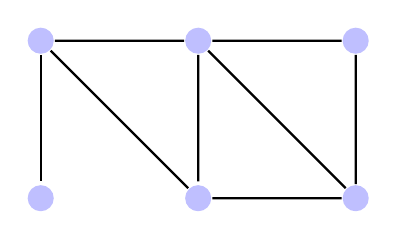
\begin{tikzpicture}[shorten >=1pt,auto,node distance=2cm,thick,main node/.style={circle,fill=blue!25}]                      
  \node[main node] (a) {};                                                                                                  
  \node[main node] (b) [left of=a] {};                                                                                      
  \node[main node] (c) [below of=a] {};                                                                                     
  \node[main node] (d) [left of=b] {};                                                                                      
  \node[main node] (e) [below of=b] {};                                                                                     
  \node[main node] (f) [below of=d] {};                                                                                     
                                                                                                                            
  \draw (c) -- (a) -- (b) -- (c) -- (e) -- (d) -- (b) -- (e);                                                               
  \draw (d) -- (f);                                                                                                         
\end{tikzpicture}
